\documentclass{standalone}
\usepackage{tikz}
\usetikzlibrary{patterns, positioning}


\begin{document}
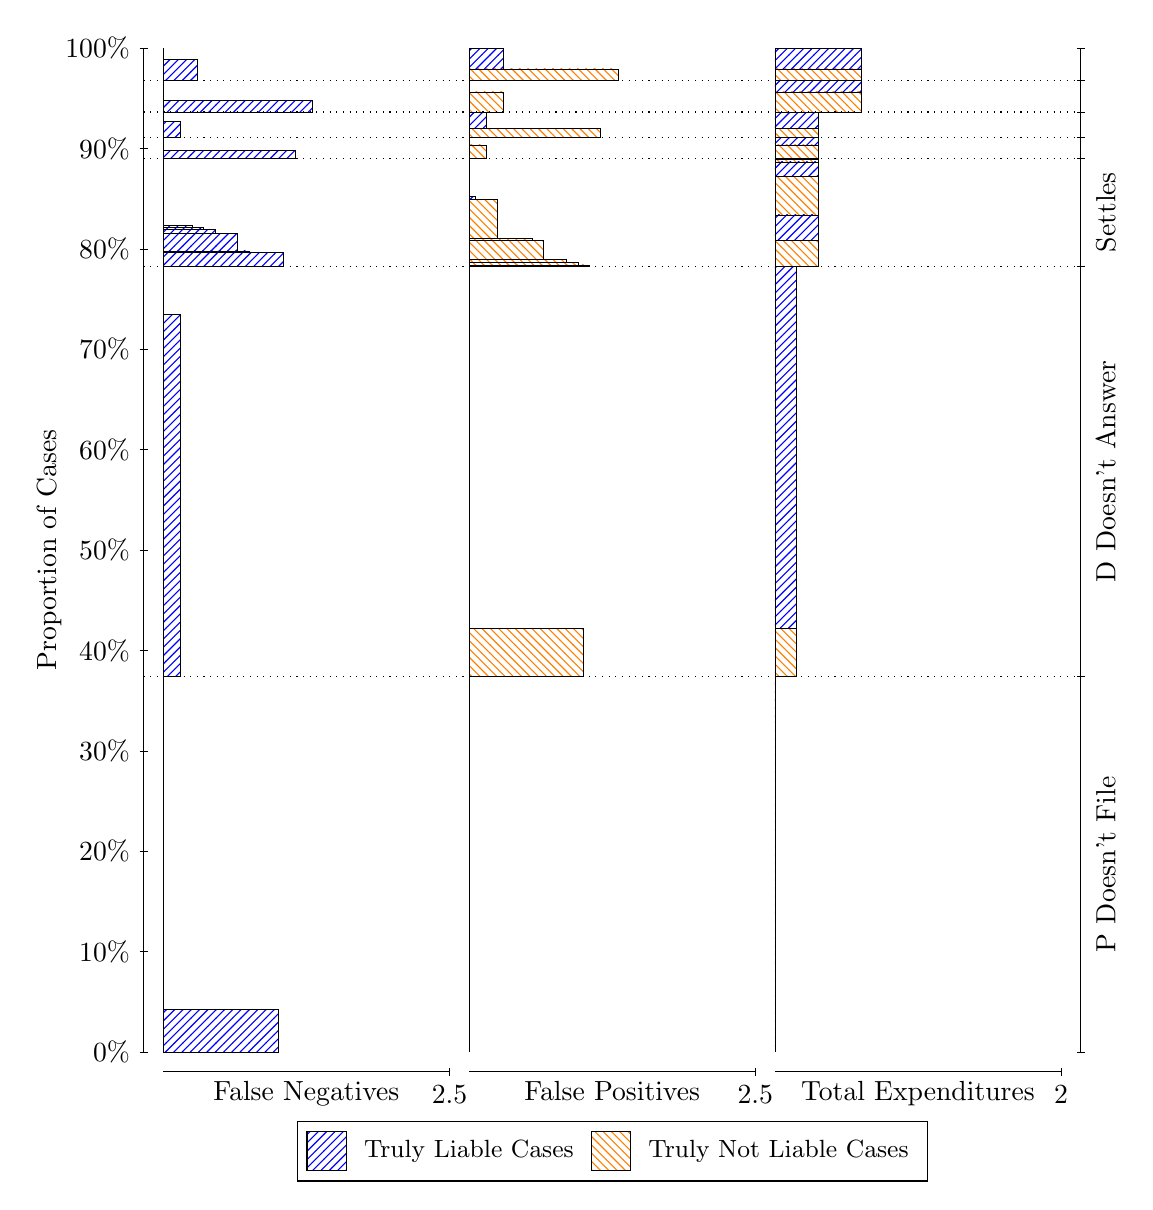
\begin{tikzpicture}
\draw[black, very thin] (1.5,1.75) -- (1.5,14.5);
\node[rotate=90, text=black, anchor=center] at (0.3, 8.125) {Proportion of Cases};
\draw[black, very thin] (1.45,1.75) -- (1.55,1.75);
\node[text=black, anchor=east] at (1.45, 1.75) {0\%};
\draw[black, very thin] (1.45,3.025) -- (1.55,3.025);
\node[text=black, anchor=east] at (1.45, 3.025) {10\%};
\draw[black, very thin] (1.45,4.3) -- (1.55,4.3);
\node[text=black, anchor=east] at (1.45, 4.3) {20\%};
\draw[black, very thin] (1.45,5.575) -- (1.55,5.575);
\node[text=black, anchor=east] at (1.45, 5.575) {30\%};
\draw[black, very thin] (1.45,6.85) -- (1.55,6.85);
\node[text=black, anchor=east] at (1.45, 6.85) {40\%};
\draw[black, very thin] (1.45,8.125) -- (1.55,8.125);
\node[text=black, anchor=east] at (1.45, 8.125) {50\%};
\draw[black, very thin] (1.45,9.4) -- (1.55,9.4);
\node[text=black, anchor=east] at (1.45, 9.4) {60\%};
\draw[black, very thin] (1.45,10.675) -- (1.55,10.675);
\node[text=black, anchor=east] at (1.45, 10.675) {70\%};
\draw[black, very thin] (1.45,11.95) -- (1.55,11.95);
\node[text=black, anchor=east] at (1.45, 11.95) {80\%};
\draw[black, very thin] (1.45,13.225) -- (1.55,13.225);
\node[text=black, anchor=east] at (1.45, 13.225) {90\%};
\draw[black, very thin] (1.45,14.5) -- (1.55,14.5);
\node[text=black, anchor=east] at (1.45, 14.5) {100\%};

\draw[black, very thin] (13.4,1.75) -- (13.4,14.5);
\draw[black, very thin] (13.35,1.75) -- (13.45,1.75);
\node[anchor=west] at (13.35, 1.75) {};
\draw[black, very thin] (13.35,6.5185) -- (13.45,6.5185);
\node[anchor=west] at (13.35, 6.5185) {};
\draw[black, very thin] (13.35,11.731) -- (13.45,11.731);
\node[anchor=west] at (13.35, 11.731) {};
\draw[black, very thin] (13.35,13.102) -- (13.45,13.102);
\node[anchor=west] at (13.35, 13.102) {};
\draw[black, very thin] (13.35,13.367) -- (13.45,13.367);
\node[anchor=west] at (13.35, 13.367) {};
\draw[black, very thin] (13.35,13.687) -- (13.45,13.687);
\node[anchor=west] at (13.35, 13.687) {};
\draw[black, very thin] (13.35,14.088) -- (13.45,14.088);
\node[anchor=west] at (13.35, 14.088) {};
\draw[black, very thin] (13.35,14.5) -- (13.45,14.5);
\node[anchor=west] at (13.35, 14.5) {};

\draw[black, very thin, pattern color=blue, pattern=north east lines] (1.75,1.75) rectangle (3.2033,2.2911);
\draw[black, very thin, pattern color=orange, pattern=north west lines] (1.75,2.2911) rectangle (1.75,6.5185);
\draw[black, very thin, pattern color=blue, pattern=north east lines] (1.75,6.5185) rectangle (1.968,11.122);
\draw[black, very thin, pattern color=orange, pattern=north west lines] (1.75,11.122) rectangle (1.75,11.731);
\draw[black, very thin, pattern color=blue, pattern=north east lines] (1.75,11.731) rectangle (3.276,11.909);
\draw[black, very thin, pattern color=blue, pattern=north east lines] (1.75,11.909) rectangle (2.84,11.925);
\draw[black, very thin, pattern color=blue, pattern=north east lines] (1.75,11.925) rectangle (2.6947,12.15);
\draw[black, very thin, pattern color=blue, pattern=north east lines] (1.75,12.15) rectangle (2.404,12.196);
\draw[black, very thin, pattern color=blue, pattern=north east lines] (1.75,12.196) rectangle (2.2587,12.222);
\draw[black, very thin, pattern color=blue, pattern=north east lines] (1.75,12.222) rectangle (2.1133,12.251);
\draw[black, very thin, pattern color=orange, pattern=north west lines] (1.75,12.251) rectangle (1.75,13.102);
\draw[black, very thin, pattern color=blue, pattern=north east lines] (1.75,13.102) rectangle (3.4213,13.197);
\draw[black, very thin, pattern color=orange, pattern=north west lines] (1.75,13.197) rectangle (1.75,13.367);
\draw[black, very thin, pattern color=blue, pattern=north east lines] (1.75,13.367) rectangle (1.968,13.571);
\draw[black, very thin, pattern color=orange, pattern=north west lines] (1.75,13.571) rectangle (1.75,13.687);
\draw[black, very thin, pattern color=blue, pattern=north east lines] (1.75,13.687) rectangle (3.6393,13.832);
\draw[black, very thin, pattern color=orange, pattern=north west lines] (1.75,13.832) rectangle (1.75,14.088);
\draw[black, very thin, pattern color=blue, pattern=north east lines] (1.75,14.088) rectangle (2.186,14.353);
\draw[black, very thin, pattern color=orange, pattern=north west lines] (1.75,14.353) rectangle (1.75,14.5);
\draw[black, very thin, pattern color=orange, pattern=north west lines] (5.6333,1.75) rectangle (5.6333,5.9775);
\draw[black, very thin, pattern color=blue, pattern=north east lines] (5.6333,5.9775) rectangle (5.6333,6.5185);
\draw[black, very thin, pattern color=orange, pattern=north west lines] (5.6333,6.5185) rectangle (7.0867,7.1273);
\draw[black, very thin, pattern color=blue, pattern=north east lines] (5.6333,7.1273) rectangle (5.6333,11.731);
\draw[black, very thin, pattern color=orange, pattern=north west lines] (5.6333,11.731) rectangle (7.1593,11.747);
\draw[black, very thin, pattern color=orange, pattern=north west lines] (5.6333,11.747) rectangle (7.014,11.773);
\draw[black, very thin, pattern color=orange, pattern=north west lines] (5.6333,11.773) rectangle (6.8687,11.819);
\draw[black, very thin, pattern color=orange, pattern=north west lines] (5.6333,11.819) rectangle (6.578,12.054);
\draw[black, very thin, pattern color=orange, pattern=north west lines] (5.6333,12.054) rectangle (6.4327,12.087);
\draw[black, very thin, pattern color=orange, pattern=north west lines] (5.6333,12.087) rectangle (5.9967,12.581);
\draw[black, very thin, pattern color=blue, pattern=north east lines] (5.6333,12.581) rectangle (5.706,12.611);
\draw[black, very thin, pattern color=blue, pattern=north east lines] (5.6333,12.611) rectangle (5.6333,13.102);
\draw[black, very thin, pattern color=orange, pattern=north west lines] (5.6333,13.102) rectangle (5.8513,13.271);
\draw[black, very thin, pattern color=blue, pattern=north east lines] (5.6333,13.271) rectangle (5.6333,13.367);
\draw[black, very thin, pattern color=orange, pattern=north west lines] (5.6333,13.367) rectangle (7.3047,13.482);
\draw[black, very thin, pattern color=blue, pattern=north east lines] (5.6333,13.482) rectangle (5.8513,13.687);
\draw[black, very thin, pattern color=orange, pattern=north west lines] (5.6333,13.687) rectangle (6.0693,13.943);
\draw[black, very thin, pattern color=blue, pattern=north east lines] (5.6333,13.943) rectangle (5.6333,14.088);
\draw[black, very thin, pattern color=orange, pattern=north west lines] (5.6333,14.088) rectangle (7.5227,14.235);
\draw[black, very thin, pattern color=blue, pattern=north east lines] (5.6333,14.235) rectangle (6.0693,14.5);
\draw[black, very thin, pattern color=orange, pattern=north west lines] (9.5167,1.75) rectangle (9.5167,5.9775);
\draw[black, very thin, pattern color=blue, pattern=north east lines] (9.5167,5.9775) rectangle (9.5167,6.5185);
\draw[black, very thin, pattern color=orange, pattern=north west lines] (9.5167,6.5185) rectangle (9.7892,7.1273);
\draw[black, very thin, pattern color=blue, pattern=north east lines] (9.5167,7.1273) rectangle (9.7892,11.731);
\draw[black, very thin, pattern color=orange, pattern=north west lines] (9.5167,11.731) rectangle (10.062,12.054);
\draw[black, very thin, pattern color=blue, pattern=north east lines] (9.5167,12.054) rectangle (10.062,12.381);
\draw[black, very thin, pattern color=orange, pattern=north west lines] (9.5167,12.381) rectangle (10.062,12.875);
\draw[black, very thin, pattern color=blue, pattern=north east lines] (9.5167,12.875) rectangle (10.062,13.053);
\draw[black, very thin, pattern color=orange, pattern=north west lines] (9.5167,13.053) rectangle (10.062,13.086);
\draw[black, very thin, pattern color=blue, pattern=north east lines] (9.5167,13.086) rectangle (10.062,13.102);
\draw[black, very thin, pattern color=orange, pattern=north west lines] (9.5167,13.102) rectangle (10.062,13.271);
\draw[black, very thin, pattern color=blue, pattern=north east lines] (9.5167,13.271) rectangle (10.062,13.367);
\draw[black, very thin, pattern color=orange, pattern=north west lines] (9.5167,13.367) rectangle (10.062,13.482);
\draw[black, very thin, pattern color=blue, pattern=north east lines] (9.5167,13.482) rectangle (10.062,13.687);
\draw[black, very thin, pattern color=orange, pattern=north west lines] (9.5167,13.687) rectangle (10.607,13.943);
\draw[black, very thin, pattern color=blue, pattern=north east lines] (9.5167,13.943) rectangle (10.607,14.088);
\draw[black, very thin, pattern color=orange, pattern=north west lines] (9.5167,14.088) rectangle (10.607,14.235);
\draw[black, very thin, pattern color=blue, pattern=north east lines] (9.5167,14.235) rectangle (10.607,14.5);
\draw[black, dotted] (1.5,6.5185) -- (13.4,6.5185);
\draw[black, dotted] (1.5,11.731) -- (13.4,11.731);
\draw[black, dotted] (1.5,13.102) -- (13.4,13.102);
\draw[black, dotted] (1.5,13.367) -- (13.4,13.367);
\draw[black, dotted] (1.5,13.687) -- (13.4,13.687);
\draw[black, dotted] (1.5,14.088) -- (13.4,14.088);
\draw[black, very thin] (1.75,1.5) -- (5.3833,1.5);
\node[text=black, anchor=north] at (3.5667, 1.5) {False Negatives};
\draw[black, very thin] (5.3833,1.45) -- (5.3833,1.55);
\node[text=black, anchor=north] at (5.3833, 1.45) {2.5};

\draw[black, very thin] (5.6333,1.5) -- (9.2667,1.5);
\node[text=black, anchor=north] at (7.45, 1.5) {False Positives};
\draw[black, very thin] (9.2667,1.45) -- (9.2667,1.55);
\node[text=black, anchor=north] at (9.2667, 1.45) {2.5};

\draw[black, very thin] (9.5167,1.5) -- (13.15,1.5);
\node[text=black, anchor=north] at (11.333, 1.5) {Total Expenditures};
\draw[black, very thin] (13.15,1.45) -- (13.15,1.55);
\node[text=black, anchor=north] at (13.15, 1.45) {2};

\node[text=black, centered, rotate=90] at (13.72, 4.1343) {P Doesn't File};
\node[text=black, centered, rotate=90] at (13.72, 9.1246) {D Doesn't Answer};
\node[text=black, centered, rotate=90] at (13.72, 12.416) {Settles};





\draw (7.449999999999999,1.5) node[draw=none] (baseCoordinate) {};
\begin{scope}[align=center]
        \matrix[scale=0.5, draw=black, below=0.5cm of baseCoordinate, nodes={draw}, column sep=0.1cm]{
            \node[rectangle, draw, minimum width=0.5cm, minimum height=0.5cm, pattern color=blue, pattern=north east lines] {}; &
            \node[draw=none, font=\small, text=black] (B) {Truly Liable Cases}; &
            \node[rectangle, draw, minimum width=0.5cm, minimum height=0.5cm, pattern color=orange, pattern=north west lines] {}; &
            \node[draw=none, font=\small, text=black] (B) {Truly Not Liable Cases}; \\
            };
\end{scope}

\end{tikzpicture}
\end{document}